% LLM-Powered Threat Intelligence Assistant Proposal
\documentclass[10pt]{article}
\usepackage[margin=0.8in]{geometry}
\usepackage{hyperref}
\usepackage{enumitem}
\usepackage{graphicx}
\usepackage{float}
\usepackage{titlesec}
\setlist{nosep}
\titlespacing*{\section}{0pt}{*1}{*0.5}

\title{LLM-Powered Threat Intelligence Assistant on GCP}
\author{Ben Blake}
\date{June 23, 2025}

\begin{document}
\maketitle

\section*{Project Overview}
This project aims to deploy a lightweight Large Language Model (LLM) inference service for cybersecurity threat intelligence on Google Cloud Platform (GCP). The service will analyze security logs and provide threat classification, risk scoring, and summary explanations to assist security analysts in rapid threat triage and response.

\section*{LLM Strategy}
The project will leverage Google Vertex AI's Gemini API, accessed via a Cloud Run serverless wrapper. This approach utilizes a managed, scalable, and secure LLM solution within the GCP free tier, minimizing operational overhead and maximizing reliability. By using Vertex AI, the project benefits from state-of-the-art language understanding and generation capabilities without the need to manage model infrastructure or resources.

\section*{Architecture}
\begin{figure}[H]
    \centering
    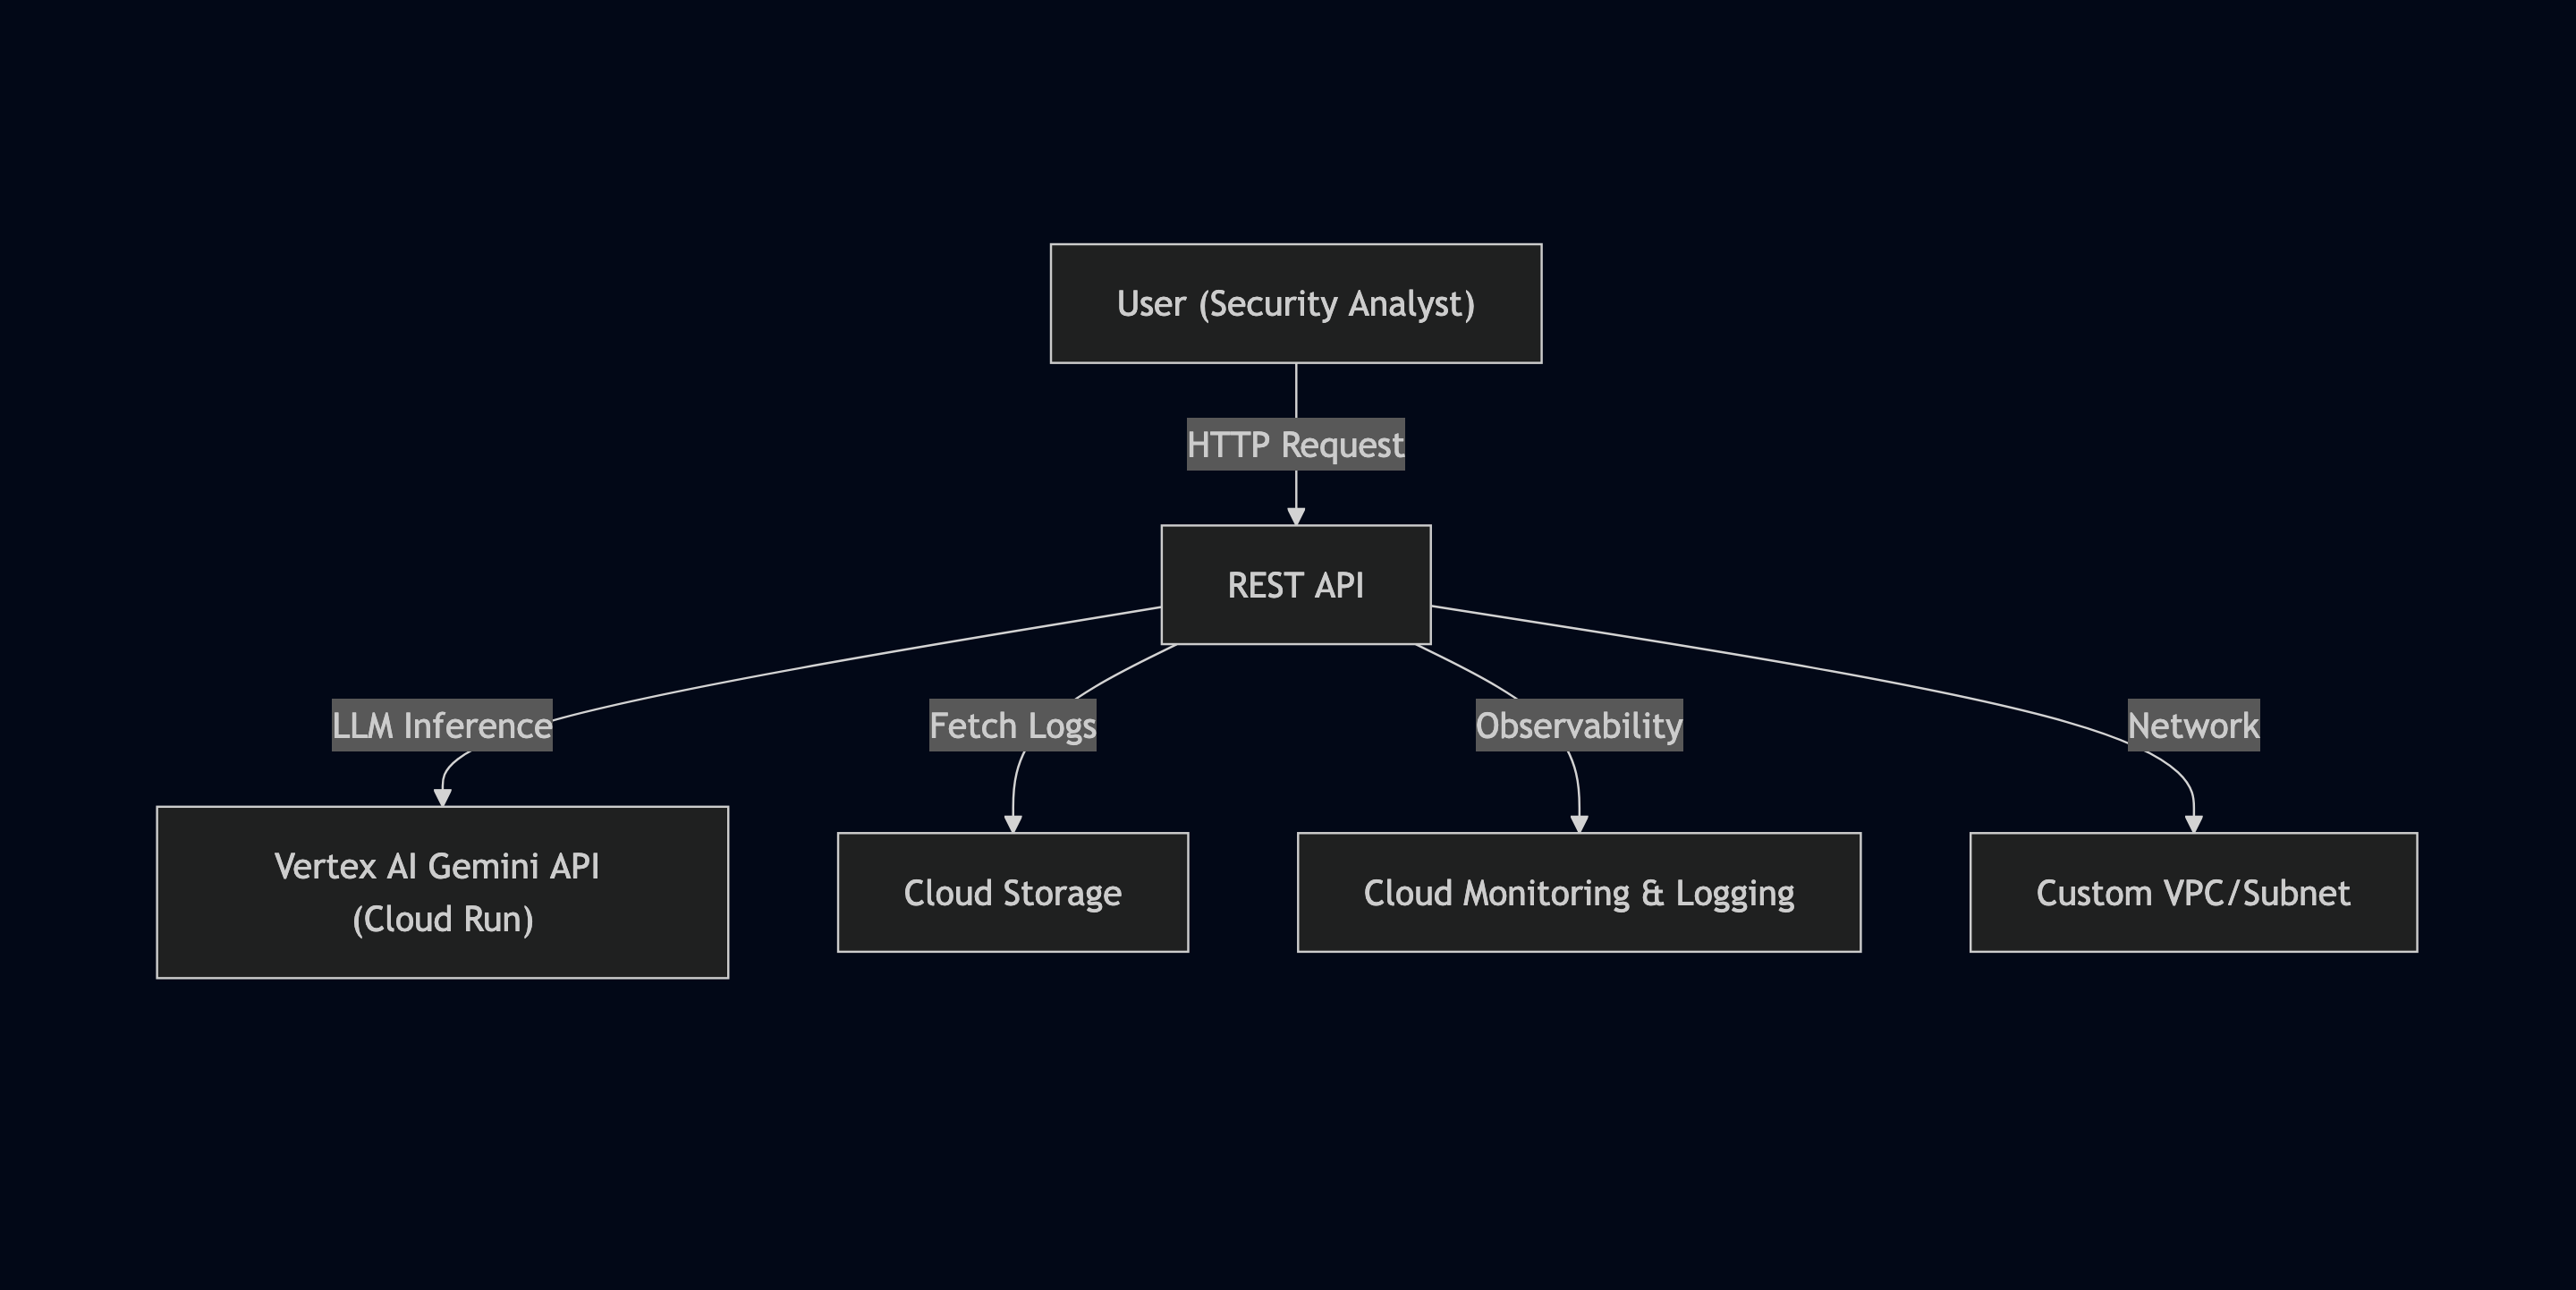
\includegraphics[width=0.7\textwidth]{images/diagram.png}
    \caption{Architecture Diagram}
    \label{fig:architecture}
\end{figure}

\section*{GCP Setup and Cost Management}
\begin{itemize}[leftmargin=*, itemsep=0.5em]
    \item New GCP project with billing enabled and \$300 free trial confirmed.
    \item All resources (VPC, subnet, firewall, Cloud Run) provisioned via Terraform.
    \item Strict adherence to Always Free tier and daily cost monitoring.
    \item Resources destroyed after each session to avoid unnecessary charges.
\end{itemize}

\section*{Git Repository}
The Terraform code, screenshots, and documentation for this project are available at:
\begin{itemize}
    \item \textbf{GitHub Repository:} \url{https://github.com/blakeben/llm-project-2025}
\end{itemize}

\end{document} 